\documentclass[UTF8]{ctexart}

%\usepackage{indentfirst}           % 首行缩进 
\usepackage[a4paper, left = 3cm, right = 3cm]{geometry}
\usepackage[bf]{titlesec}
\usepackage{listings}               % 代码环境
\usepackage{sverb}
\usepackage{xcolor}
\lstset{numbers = left,             % 设置行号位置
        numberstyle = \tiny,        % 设置行号大小
        keywordstyle = \color{blue!70},                         % 设置关键字颜色
        commentstyle = \color{red!50!green!50!blue!50},         % 设置注释颜色
        frame = single,             % 设置边框格式
        rulesepcolor = \color{red!20!green!20!blue!20},
        escapeinside = ',          % 逃逸字符,用于显示中文
        xleftmargin = 1em, xrightmargin = 1em, aboveskip = 1em, % 设置边框边距        
        tabsize = 4,                % 设置tab空格数
        showspaces = false,         % 不显示空格
        extendedchars = false,
        flexiblecolumns,            % 字列非等宽
        breaklines                  % 自动将长代码换行排版
        }

\usepackage[colorlinks, linkcolor = black, anchorcolor = black, citecolor = black]{hyperref}            % 目录超链接
\renewcommand{\contentsname}{\centerline{目录}}
\usepackage[nottoc]{tocbibind}      % 章节编号等加入目录
\usepackage{ctex}
\usepackage{graphicx}               % 插图    
\usepackage{subfigure}              % 实现图片并排
\usepackage{float}                  % 强制图片位置
\usepackage{amsmath}                % 数学公式  
\usepackage{fancyvrb}

\usepackage{fancyhdr}                   % 设置页眉页脚
\pagestyle{fancy}
\lhead{编码引论第三次仿真实验报告}
\chead{}
\rhead{无35 \quad 陈馨瑶 \quad 2013011166}
\lfoot{}
\cfoot{\thepage}
\rfoot{}

%\title{\vspace*{6cm}编码引论第三次仿真实验报告}
\title{编码引论第三次仿真实验报告}
\author{无35 \quad 陈馨瑶 \quad 2013011166}
\date{\today}

\begin{document}

%\begin{titlepage}
\maketitle

%\thispagestyle{empty}
%\end{titlepage}

\setlength{\headheight}{13pt}

%\tableofcontents

%\newpage

\section{分工}

本次实验的分工如下:

\subsection{PART I 量化}

\begin{itemize}
    \item 画 R-D 曲线图。设计 4 个不同步长的均匀量化器,将其比特率,PSNR 绘制在 R-D 图中,用线段
连接。横轴为比特率,纵轴为 PSNR。
    \item 练习 JPEG/H.261 量化器,绘制 R-D 图。
    \item 设计非均匀量化器,绘制 R-D 图。
    \item 对三类量化器进行评价。
\end{itemize}

\subsection{PART II 变长编码(独立符号)}

\begin{itemize}
    \item 设计变长编码器,用变长码对量化后的图象编码。输入符号(象素)进行独立编码。
    \item 给出编码前后的比特数,计算压缩比。
\end{itemize}

\subsection{PART III 变长编码(两符号联合)}

\begin{itemize}
    \item 设计变长编码器,用变长码对量化后的图象编码。输入符号(象素)进行独立编码。
    \item 给出编码前后的比特数,计算压缩比。
\end{itemize}

其中,由我完成的是第二部分:变长编码(独立符号),由于各部分实验内容较为独立,故而在模块实现部分仅对我自己完成的内容进行了总结。

\section{模块实现}

所采用的熵编码为Huffman码,原理在书上和课件上都有所讲解。实验时,统一均匀量化,步长为20,则量化后的灰度值只可能是10, 30, 50……Huffman码利用不同符号的概率进行编码,在这里的概率即具体图像中不同灰度值所占的比率。为简化计算,我编写了如下的程序计算编码:

\lstinputlisting[language = Matlab]{Huffman.m}

\section{实验结果}

\subsection{PART I 量化}

\footnote{本部分完成人:刘家硕}用H261,两侧细化和中部细化三种量化器分别和均匀量化进行比较,结果如下:
\begin{figure}[H]
    \centering
    \includegraphics[width = \textwidth]{02.png}
\end{figure}

H261和两侧细化量化器的R-D曲线分别如下:
\begin{figure}[H]
    \centering
    \includegraphics[width = \textwidth]{03.png}
\end{figure}

\begin{figure}[H]
    \centering
    \includegraphics[width = \textwidth]{04.png}
\end{figure}

据此,对三类量化器的评价如下:

H261比均匀量化好很多,尝试的两种非均匀量化方式和均匀量化相比几乎没有区别,最优的非均匀量化应该是重建数值在量化区间重心,量化区间边界在重建数值中点的情况,由于软件设计的是重建数值为量化区间中值故无法实现最优。

\subsection{PART II 变长编码(独立符号)}

()最后得到的VLC码表如下:

\verbinput{huffman.txt}

编码前(量化后)和编码后的图像对比如下:

\begin{figure}[H]
    \centering
    \subfigure[编码前图像]{
    \includegraphics[scale = 1.0]{1.png}}
    \hspace{\bigskipamount}
    \subfigure[编码后图像]{
    \includegraphics[scale = 1.0]{huffman.png}}
    \caption{编码前后图像对比}
\end{figure}

从上图可以看出,解码后的图像成功恢复了原有图像,二者并无差别。编码前图像为131072bit,量化与编码后为52643bit,压缩比为40.16\%。

对Huffman码的评价:作为一种熵编码,能在不丢失信息的同时达到这样的压缩比,说明这种编码是较为有效的。但我认为其可能存在问题在于实现上,由于每一步都需要对符号的概率进行排序,在信源符号数较多时会带来较大的计算复杂度,并且要直到最后一步才能向前倒推编码,所以在实现时也存在存储的问题。


\subsection{PART III 变长编码(两符号联合)}

\footnote{本部分完成人:李思涵} 同样采用均匀量化,步长20,得到的结果如下:
\begin{figure}[H]
    \centering
    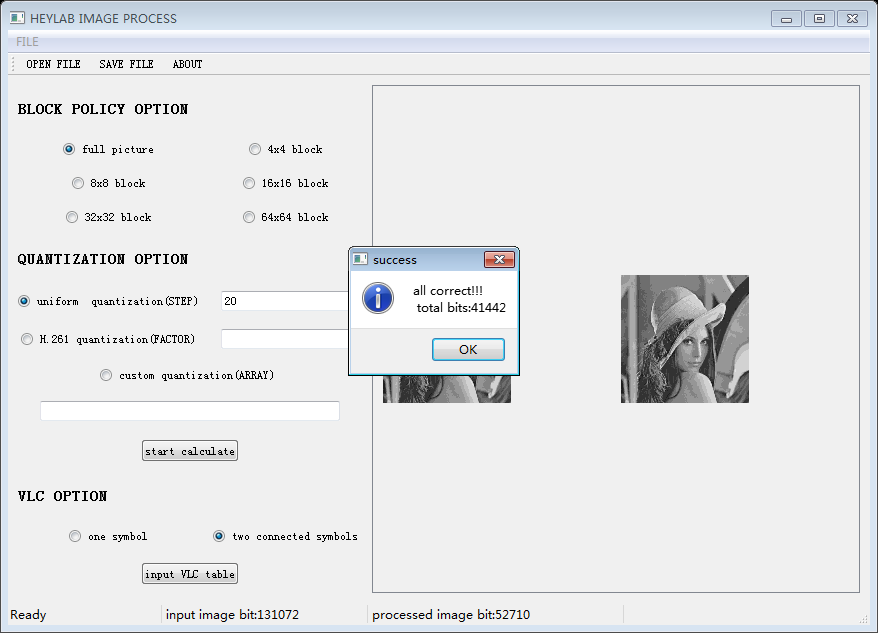
\includegraphics[width = \textwidth]{result.png}
\end{figure}

可以看出采用两符号联合方式编码的压缩比是小于独立符号编码的。

\end{document}